\paragraph{Desarrollo técnico}
\paragraph{}
la idea original del proyecto fue el realizar un transmisor y receptor de FM digital. El sistema se pensó de forma que su frecuencia de trabajo fuera aproximadamente 1MHz. 
El transmisor modulaba la frecuencia portadora de forma que una tensión inversa de baja frecuencia (moduladora), se aplicaba a unos diodos capacitivos o varactores. Estos diodos varactores se encontraban de circuito tanque en el bucle de oscilación.
Este modelo de transmisor funcionaba correctamente.

\paragraph{}
Por otro lado, el receptor de FM era bastante complejo. Un filtro de entrada exigente, seguido de un amplificador, y acontinuación una etapa de filtrado muy agudo a la frecuencia de la portadora. Esta estrategia permite la conversión de una señal modulada en FM a una señal modulada en AM. Posteriormente se realizala etapa del demodulador AM el cual requería de amplificadores y acondicionamiento de señal tedioso.  
%ANADIR IMAGENES BUSCAR
\begin{figure}[h]
    \centering
    \includegraphics[scale=.3, width=.3\textwidth]{crono_tx_rx_osciloscopio}
    \caption{Primer emisor y receptor montados en placa de entrenamiento}
    \label{fig:crono_tx_rx_osciloscopio}
\end{figure}

\begin{figure}[h]
    \centering
    \includegraphics[scale=.3, width=.3\textwidth]{crono_2tx_placa}
    \caption{Modelos de transmisores soldados placa}
    \label{fig:crono_2tx_placa}
\end{figure}

\begin{figure}[h]
    \centering
    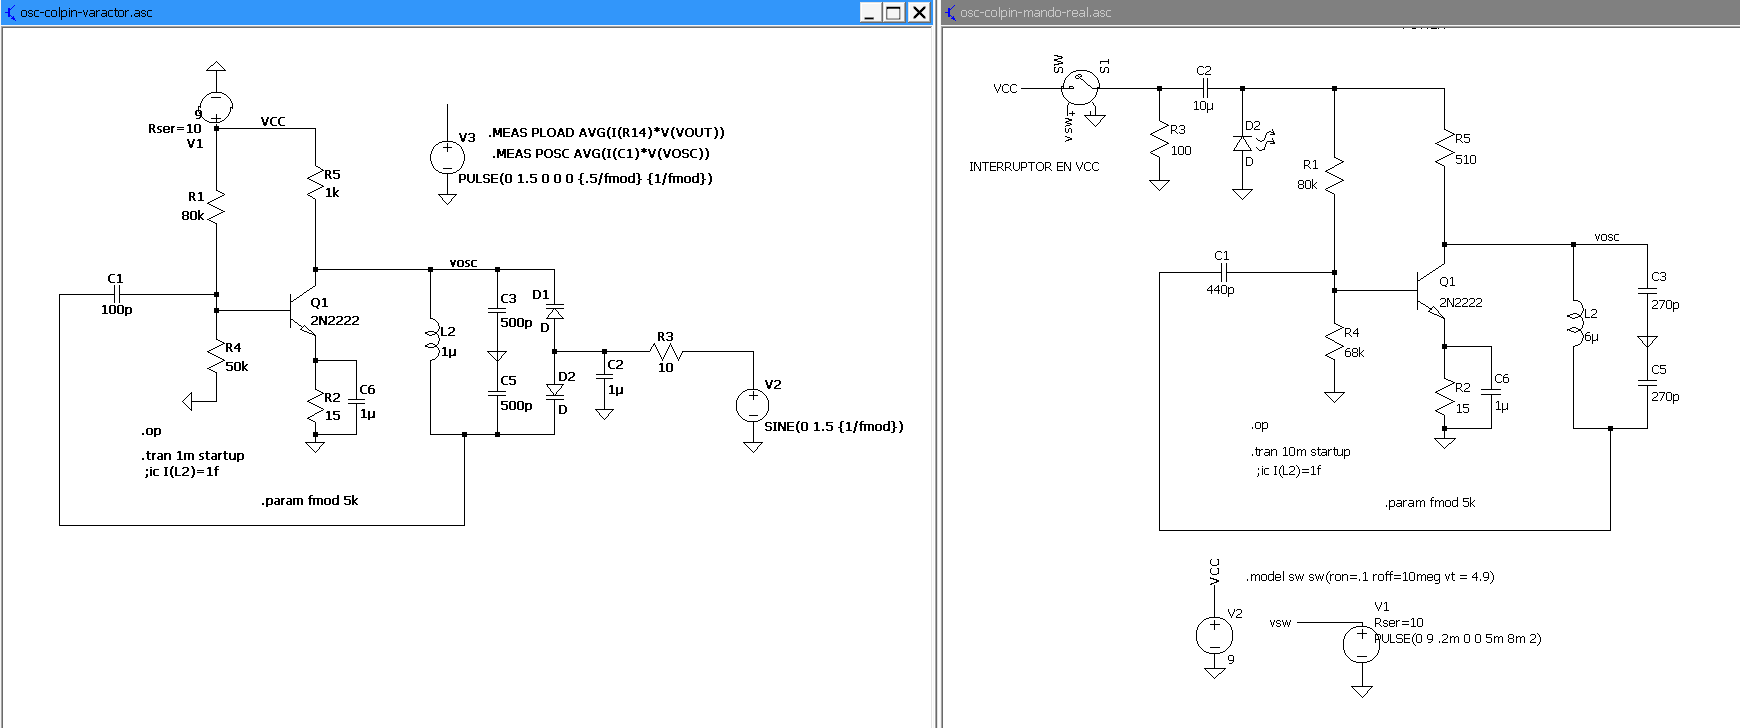
\includegraphics[scale=1, width=1\textwidth]{crono_sch_varactor_tx}
    \caption{Modelos esquemáticos de transmisores} 
    \label{fig:crono_sch_varactor_tx}
\end{figure}

\paragraph{Motivos de reemplazo}
\paragraph{}
Los motivos de remplazo de este modelo fueron varios.
En primer lugar, el sistema de transmisor y receptor no funcionaba a distancias mayores de pocos centímetros. Esto era debido principalmente a la baja potencia radiada. La bobina del circuito tanque de oscilación debía tener numerosas espiras para que a esa frecuencia tan baja consiguiera inducir, por acople magnético, tensión en el receptor.
A parte de el problema mencionado, el transmisor tenía un excesivo consumo estático. En cuanto al receptor, los problemas también fueron varios. Los filtros, tan agudos eran complicados de fabricar, más si los filtros debían ser diseñados a la frecuencia de la portadora como conversión directa. Además, la necesidad de implementar también el demodulador de AM tomando como entrada la señal filtrada se hacía complicado.
Finalmente se opta por mejorar el diseño del sistema proponiendo una segunda versión.
